\documentclass[11pt,oneside]{report}
\usepackage[utf8]{inputenc}
\usepackage[T1]{fontenc}
\usepackage{mathptmx,microtype,geometry,xcolor,graphicx,booktabs,longtable,array,tabularx}
\geometry{a4paper,margin=24mm,headheight=15pt}
\usepackage{tikz}
\usetikzlibrary{arrows.meta,positioning,shapes.geometric}
\usepackage[most]{tcolorbox}
\usepackage{listings,fancyhdr,hyperref}
\definecolor{nexora}{HTML}{285FCA}
\hypersetup{colorlinks=true,linkcolor=nexora,urlcolor=nexora,citecolor=nexora,pdftitle={Nexora : documentation technique et pédagogique}}
\pagestyle{fancy}\fancyhf{}\fancyhead[L]{\small Nexora / CNC Platform}\fancyhead[R]{\small Documentation technique}\fancyfoot[C]{\thepage}
\setlength{\parindent}{0pt}\setlength{\parskip}{5pt}\setcounter{tocdepth}{1}
\renewcommand{\contentsname}{Table des matières}\renewcommand{\listfigurename}{Liste des figures}\renewcommand{\listtablename}{Liste des tableaux}\renewcommand{\bibname}{Références officielles}\renewcommand{\chaptername}{Chapitre}
\newtcolorbox{concept}[1]{breakable,colback=blue!3,colframe=nexora,title=#1,fonttitle=\bfseries}
\lstdefinelanguage{TypeScript}{keywords={import,from,export,async,await,const,let,return,if,else,throw,new,function,interface,type,try,catch},sensitive=true,morecomment=[l]{//},morestring=[b]',morestring=[b]"}
\lstset{language=TypeScript,basicstyle=\ttfamily\scriptsize,breaklines=true,columns=fullflexible,keepspaces=true,numbers=left,numberstyle=\tiny\color{gray},numbersep=7pt,frame=single,rulecolor=\color{blue!15},keywordstyle=\color{nexora},commentstyle=\color{gray},showstringspaces=false,extendedchars=true,literate={é}{{\'e}}1 {è}{{\`e}}1 {ê}{{\^e}}1 {à}{{\`a}}1 {â}{{\^a}}1 {î}{{\^i}}1 {ô}{{\^o}}1 {û}{{\^u}}1 {ù}{{\`u}}1 {ç}{{\c c}}1 {É}{{\'E}}1 {œ}{{\oe}}1 {’}{{'}}1 {—}{{---}}1 {→}{{$\rightarrow$}}1 {…}{{...}}1 {·}{{$\cdot$}}1 {”}{{"}}1 {€}{{EUR}}1}
\emergencystretch=3em

\begin{document}
\hypersetup{pageanchor=false}
\begin{titlepage}
\color{nexora}\rule{\textwidth}{3pt}\vspace{2cm}
{\Huge\bfseries NEXORA\par}\vspace{0.5cm}{\Large CNC Platform\par}
\vspace{1.5cm}{\huge Documentation technique\par et pédagogique\par}
\vspace{1cm}{\large Architecture, données, sécurité\par et guide de développement\par}
\vfill\color{black}Projet CPGE / préparation aux concours\par
État du code au 12 novembre 2026\par Dépôt : achraflm/Nexora-cpge\par
\vspace{1cm}\rule{\textwidth}{0.5pt}
\small Ce rapport décrit le code observé. Les composants de démonstration, les routes inachevées et les limites de déploiement sont distingués des fonctions vérifiées.
\end{titlepage}
\pagenumbering{roman}
\hypersetup{pageanchor=true}
\tableofcontents\listoffigures\listoftables
\clearpage\pagenumbering{arabic}
\chapter{Présentation générale et périmètre vérifié}
\section{Objectif et public}
Nexora accompagne la préparation CPGE : cours, travaux dirigés, annales et suivi du travail. Le problème traité est la dispersion des documents et des activités de révision. Le projet combine une interface académique et un backend organisé par domaines. Le nouveau catalogue couvre exclusivement MPSI/SUP et MP/SPE, avec Mathématiques, Physique-Chimie, Informatique et SII. Les anciens modules et comptes peuvent encore utiliser MP, PSI et TSI : cette coexistence est visible dans le code.

\section{Méthode de lecture}
L’analyse porte sur les sources applicatives, manifestes de dépendances, six schémas Prisma, routes Express et Next.js, tests et configuration Docker. Les dépendances installées et archives ne sont pas des sources métier. Les extraits proviennent des fichiers réels et leurs lignes et empreintes sont conservées dans verification/extraits.json. Les raisons techniques proposées sont des analyses de compromis, pas des intentions historiques attribuées aux auteurs.

\begin{table}[ht]\centering\small\begin{tabularx}{\textwidth}{lX}\toprule Fonction & État constaté \\\midrule
Authentification & Inscription, connexion, cookie privé, rôles et révocation branchés au backend. \\
Tableau de bord & Lecture réelle des activités ; radar, objectifs et calendrier. Activités artificielles pour les comptes démo. \\
Ressources & Import, brouillons, publication, filtres, stockage privé et lecteur PDF opérationnels. \\
Conversion & DOC, DOCX, PPT, PPTX et TEX convertis en conteneur isolé et testés. \\
Cours historiques & Interfaces et catalogue externe ; plusieurs routes natives encore 501. \\
Examens, contact & Modèles et interfaces présents ; routes métier principales encore 501. \\
QCM adaptatif & Algorithme pur testé ; orchestration HTTP des sessions encore 501. \\
Redis / MinIO & Infrastructure déclarée ; pas de cache ni de stockage S3 actif dans le nouveau parcours. \\\bottomrule\end{tabularx}\caption{État fonctionnel vérifié}\end{table}
\section{Besoins non fonctionnels}
La confidentialité des brouillons impose une autorisation sur les métadonnées et les octets. La réactivité impose de répondre à l’import avant la fin des conversions. La sécurité impose de ne pas compiler LaTeX dans le processus principal. Une erreur de compilation doit rester attachée à son document sans faire disparaître le catalogue. La maintenance demande de distinguer affichage, protocole HTTP, règles métier et persistance.

\chapter{Architecture et circulation des requêtes}
\section{Organisation par domaines}
Next.js utilise des composants serveur pour la session et des composants client pour l’interaction. Le backend est un workspace npm contenant une gateway et six services Express. Chaque service possède son client Prisma et son schéma PostgreSQL. La séparation est logique dans une base unique ; elle ne prouve pas un déploiement distribué. common mutualise les erreurs, le contexte utilisateur et le démarrage HTTP.

\begin{figure}[ht]\centering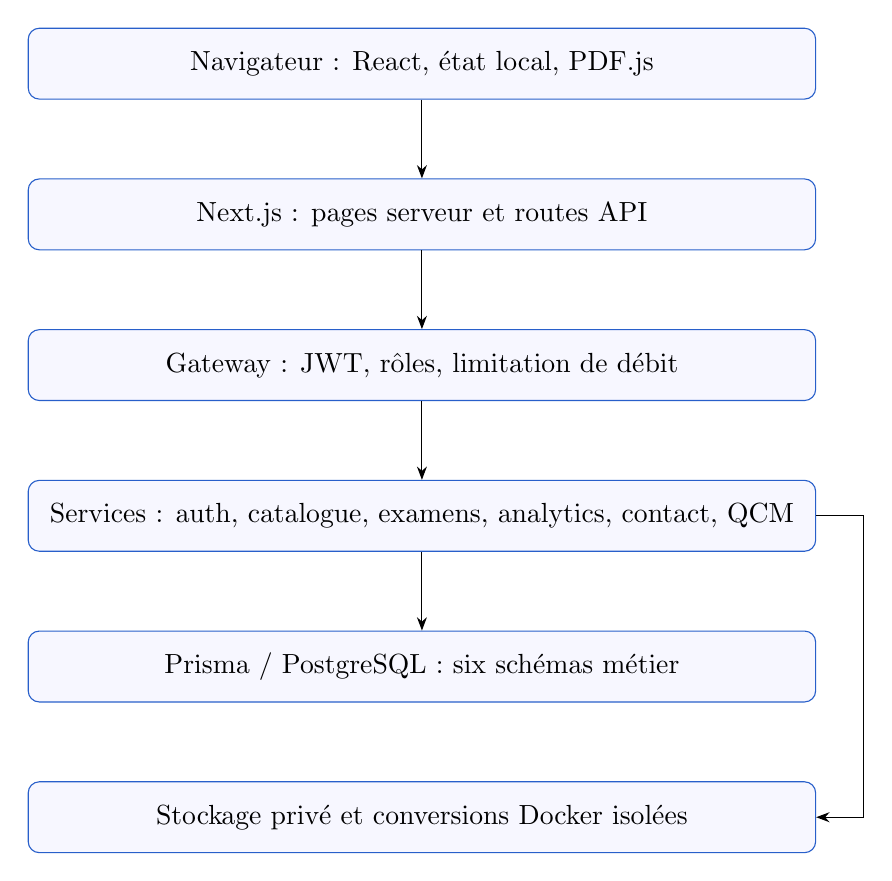
\begin{tikzpicture}[node distance=10mm,box/.style={draw=nexora,rounded corners,fill=blue!3,minimum width=10cm,minimum height=9mm,align=center},>=Stealth]
\node[box](b){Navigateur : React, état local, PDF.js};\node[box,below=of b](n){Next.js : pages serveur et routes API};\node[box,below=of n](g){Gateway : JWT, rôles, limitation de débit};\node[box,below=of g](s){Services : auth, catalogue, examens, analytics, contact, QCM};\node[box,below=of s](d){Prisma / PostgreSQL : six schémas métier};\node[box,below=of d](c){Stockage privé et conversions Docker isolées};\draw[->](b)--(n);\draw[->](n)--(g);\draw[->](g)--(s);\draw[->](s)--(d);\draw[->](s.east)--++(0.6,0)|-(c.east);\end{tikzpicture}\caption{Architecture des parcours reliés}\end{figure}
\section{Couches et responsabilités}
Les Route Handlers Next sont un backend pour le frontend : lecture du cookie, obtention d’un access token et relais autorisé. La gateway transmet le multipart sans le parser. Les routes catalogue valident les données et le rôle. resource-files.ts vérifie et stocke les octets ; resource-converter.ts traite les conversions. Prisma traduit les appels typés en SQL. Il n’existe pas de Repository/DAO uniforme ni de MVC Java à inventer.

\paragraph{Code observé} backend/gateway/src/routes.ts (lignes 25 à 36).
\lstinputlisting{extraits/routing.txt}
Lecture : la fonction construit une URL depuis la configuration. Chaque objet associe un préfixe public à un service ; /api est retiré avant transfert. Le navigateur ignore les ports internes, mais la gateway devient un point de dépendance commun.

\section{Frontières de confiance}
Le navigateur est non fiable même s’il affiche ADMIN. Le relais Next vérifie la session et le service vérifie encore le rôle. x-user-id et x-user-role ne sont fiables que reconstruits par la gateway après vérification du JWT, avec refus des appels directs sans secret interne. Un secret partagé ne chiffre pas le réseau ; les ports internes doivent rester isolés en production.

\section{Lecture d’un document}
ResourceReader suit l’état de préparation. Après READY, CoursePdfReader charge une URL privée via PDF.js. Le serveur réévalue les droits avant de servir les octets. Dépublier empêche les requêtes suivantes d’un étudiant, mais ne retire pas les octets déjà transmis à son navigateur.

\chapter{Cours pratique des technologies utilisées}
\section{TypeScript}
\subsection*{Définition}
Un système de types statiques ajouté à JavaScript ; les types sont effacés à l’exécution.

\subsection*{Fonctionnement interne et concepts}
Une interface décrit une forme, une union les cas permis. Le compilateur vérifie les usages du programme, pas les valeurs envoyées par un attaquant.

\subsection*{Utilisation dans Nexora}
Point d’entrée analysé : frontend/lib/educational-resources.ts.

\paragraph{Code observé} frontend/lib/educational-resources.ts (lignes 1 à 10).
\lstinputlisting{extraits/tech-01.txt}
\subsection*{Lecture du code et exemple pratique}
Les constantes fixent les quatre matières ; l’interface décrit le contrat de lecture ; la fonction centralise les erreurs HTTP.

\subsection*{Interactions et justification technique}
Les types structurels évitent une hiérarchie de classes sans comportement. Les données réseau exigent encore Zod.

\subsection*{Limites et alternatives}
Remplacer les any restants par des contrats précis ; JavaScript seul réduit les garanties préalables.

\section{React et composants}
\subsection*{Définition}
Une description déclarative de l’interface à partir de propriétés et d’un état.

\subsection*{Fonctionnement interne et concepts}
Une mise à jour d’état recalcule la vue. Les effets synchronisent une ressource externe et leur nettoyage annule requêtes et temporisateurs devenus inutiles.

\subsection*{Utilisation dans Nexora}
Point d’entrée analysé : frontend/components/ResourceCatalog.tsx.

\paragraph{Code observé} frontend/components/ResourceCatalog.tsx (lignes 1 à 22).
\lstinputlisting{extraits/tech-02.txt}
\subsection*{Lecture du code et exemple pratique}
Les filtres sont des états ; l’effet temporise la recherche ; AbortController empêche une réponse obsolète de modifier la vue.

\subsection*{Interactions et justification technique}
Séparer lecteur et catalogue permet de réutiliser le PDF sans dupliquer les comportements. Loading, erreur et état vide sont explicites.

\subsection*{Limites et alternatives}
Les composants historiques volumineux restent à découper ; une machine à états aiderait les parcours plus complexes.

\section{Next.js App Router}
\subsection*{Définition}
Un framework liant routage par fichiers, rendu serveur et composants React interactifs.

\subsection*{Fonctionnement interne et concepts}
Les pages serveur s’exécutent avant l’envoi de la vue. Les composants client gèrent les événements ; une route API traite Request et Response sans être un composant visuel.

\subsection*{Utilisation dans Nexora}
Point d’entrée analysé : frontend/app/page.tsx.

\paragraph{Code observé} frontend/app/page.tsx (lignes 1 à 13).
\lstinputlisting{extraits/tech-03.txt}
\subsection*{Lecture du code et exemple pratique}
La page exige une session, charge le résumé analytics puis fournit ses propriétés au DashboardShell. Une panne de statistiques ne supprime pas la session.

\subsection*{Interactions et justification technique}
Les jetons restent côté serveur. Les guides installés dans node\_modules correspondent à la version du dépôt et priment pour ses API.

\subsection*{Limites et alternatives}
Le rendu dépend de la disponibilité du service auth. Une SPA séparée demanderait une autre conservation des jetons.

\section{Node.js et asynchronisme}
\subsection*{Définition}
Un environnement JavaScript serveur utilisé par Express, les scripts et le lancement des conversions.

\subsection*{Fonctionnement interne et concepts}
La boucle d’événements coordonne les entrées-sorties. Await suspend une fonction, pas tout le serveur ; un calcul CPU synchrone bloque néanmoins son thread. Spawn crée un processus distinct.

\subsection*{Utilisation dans Nexora}
Point d’entrée analysé : backend/services/catalog-course-service/src/resource-converter.ts.

\paragraph{Code observé} backend/services/catalog-course-service/src/resource-converter.ts (lignes 1 à 18).
\lstinputlisting{extraits/tech-04.txt}
\subsection*{Lecture du code et exemple pratique}
La promesse observe stdout et le code de sortie ; le timer borne la durée ; la collecte du PDF est plafonnée. Les arguments ne passent pas par un shell hôte.

\subsection*{Interactions et justification technique}
LibreOffice et TeX travaillent hors du processus Node. Leur échec reste un résultat métier.

\subsection*{Limites et alternatives}
Une file de travaux dédiée sera nécessaire en multi-instance ; un worker thread ne suffit pas à isoler un compilateur hostile.

\section{HTTP, REST et Express}
\subsection*{Définition}
HTTP échange méthodes, chemins, en-têtes et corps ; REST organise des ressources et leurs représentations.

\subsection*{Fonctionnement interne et concepts}
Express exécute les middlewares dans l’ordre. Un refus doit terminer le traitement. POST crée, PATCH modifie et GET consulte sans mutation métier volontaire.

\subsection*{Utilisation dans Nexora}
Point d’entrée analysé : backend/packages/common/src/service-app.ts.

\paragraph{Code observé} backend/packages/common/src/service-app.ts (lignes 20 à 38).
\lstinputlisting{extraits/tech-05.txt}
\subsection*{Lecture du code et exemple pratique}
Le contrôle gateway précède le JSON puis les routes ; erreurs et routes inconnues sont traitées en dernier.

\subsection*{Interactions et justification technique}
Le multipart conserve son Content-Type et sa boundary. Les codes 401, 403, 404, 409 et 413 différencient les refus.

\subsection*{Limites et alternatives}
La relance est une commande métier plutôt qu’un REST pur. OpenAPI améliorerait la génération de clients.

\section{PostgreSQL et SQL}
\subsection*{Définition}
Un système relationnel conservant les données indépendamment du processus applicatif.

\subsection*{Fonctionnement interne et concepts}
Une clé primaire identifie une ligne, une clé étrangère impose une référence, un index accélère des recherches au prix des écritures. Une transaction regroupe des changements atomiques.

\subsection*{Utilisation dans Nexora}
Point d’entrée analysé : backend/services/catalog-course-service/prisma/resource-constraints.sql.

\paragraph{Code observé} backend/services/catalog-course-service/prisma/resource-constraints.sql (lignes 1 à 6).
\lstinputlisting{extraits/tech-06.txt}
\subsection*{Lecture du code et exemple pratique}
Le bloc vérifie la présence de la contrainte puis impose les associations filière/année. Même une écriture SQL directe respecte cette règle.

\subsection*{Interactions et justification technique}
PostgreSQL garantit les invariants ; Zod donne des erreurs précoces. Les binaires restent hors des tables.

\subsection*{Limites et alternatives}
Contains devient coûteux sur un grand corpus ; recherche plein texte et pagination seront nécessaires.

\section{Prisma et persistance}
\subsection*{Définition}
Un ORM générant un client typé depuis un schéma de données.

\subsection*{Fonctionnement interne et concepts}
Le schéma décrit champs, relations, enums et index. La génération produit les méthodes ; findMany et update génèrent des requêtes paramétrées au lieu de concaténer du SQL utilisateur.

\subsection*{Utilisation dans Nexora}
Point d’entrée analysé : backend/services/catalog-course-service/prisma/schema.prisma.

\paragraph{Code observé} backend/services/catalog-course-service/prisma/schema.prisma (lignes 100 à 128).
\lstinputlisting{extraits/tech-07.txt}
\subsection*{Lecture du code et exemple pratique}
Le modèle sépare métadonnées, stockage et conversion. subjectId matérialise la relation ; revision protège contre une ancienne conversion.

\subsection*{Interactions et justification technique}
Un client par service limite les dépendances. Les userId interservices ne sont pas tous des clés étrangères.

\subsection*{Limites et alternatives}
db push ne remplace pas un historique de migrations. La documentation en ligne peut concerner une version supérieure à Prisma 6.

\section{Zod et validation}
\subsection*{Définition}
Une validation à l’exécution qui transforme des données inconnues en valeurs acceptées.

\subsection*{Fonctionnement interne et concepts}
Parse retourne une valeur validée ou lance une erreur ; strict refuse les propriétés supplémentaires ; refine exprime un invariant entre champs.

\subsection*{Utilisation dans Nexora}
Point d’entrée analysé : backend/services/catalog-course-service/src/educational-resources.ts.

\paragraph{Code observé} backend/services/catalog-course-service/src/educational-resources.ts (lignes 19 à 26).
\lstinputlisting{extraits/tech-08.txt}
\subsection*{Lecture du code et exemple pratique}
Titre et description sont bornés ; track et level sont des enums ; refine lie MPSI/SUP et MP/SPE. Le rôle ne provient pas du formulaire.

\subsection*{Interactions et justification technique}
TypeScript protège le développement ; Zod protège la frontière réseau.

\subsection*{Limites et alternatives}
Un JSON valide ne prouve pas qu’un PDF est sain : les fichiers nécessitent une inspection distincte.

\section{Bcrypt, JWT et sessions}
\subsection*{Définition}
Le hachage de mot de passe est irréversible, la signature JWT détecte la modification et un cookie transporte la session.

\subsection*{Fonctionnement interne et concepts}
Bcrypt emploie un coût et un sel. Le refresh token aléatoire est haché en base. Le serveur signe un jeton court et la gateway vérifie algorithme, émetteur et audience.

\subsection*{Utilisation dans Nexora}
Point d’entrée analysé : backend/services/auth-user-service/src/auth.service.ts.

\paragraph{Code observé} backend/services/auth-user-service/src/auth.service.ts (lignes 50 à 59).
\lstinputlisting{extraits/tech-09.txt}
\subsection*{Lecture du code et exemple pratique}
La recherche est paramétrée ; compare emploie un hash factice si le compte manque ; l’erreur est générique ; les jetons suivent la vérification.

\subsection*{Interactions et justification technique}
HttpOnly empêche la lecture du cookie en JavaScript, pas toute XSS. SameSite et Origin réduisent CSRF ; HTTPS reste requis en production.

\subsection*{Limites et alternatives}
Révoquer le refresh token ne révoque pas immédiatement un access token déjà émis. MFA et récupération de compte ne sont pas implémentés.

\section{HTML, CSS et Tailwind}
\subsection*{Définition}
HTML porte la sémantique, CSS la présentation et Tailwind des utilitaires de styles.

\subsection*{Fonctionnement interne et concepts}
Les classes responsive appliquent des règles selon la largeur ; dark change les couleurs. Labels et noms accessibles permettent clavier et lecteurs d’écran.

\subsection*{Utilisation dans Nexora}
Point d’entrée analysé : frontend/components/CoursePdfReader.tsx.

\paragraph{Code observé} frontend/components/CoursePdfReader.tsx (lignes 60 à 69).
\lstinputlisting{extraits/tech-10.txt}
\subsection*{Lecture du code et exemple pratique}
Le retour est un bouton, le titre structure le document, les classes contrôlent bordures et tailles sans ajouter de logique métier.

\subsection*{Interactions et justification technique}
Réutiliser glowing-card et ui-button conserve l’identité visuelle. Le radar a une échelle commune et une description accessible.

\subsection*{Limites et alternatives}
Le JSX compact et les classes répétées nuisent à la revue ; extraire des composants lorsque les répétitions deviennent stables.

\section{PDF.js}
\subsection*{Définition}
Un moteur interprétant les PDF et dessinant leurs pages dans le navigateur.

\subsection*{Fonctionnement interne et concepts}
Chargement, viewport et rendu canvas sont distincts. Un worker traite une partie du travail ; changer de page demande un nouvel objet de page et un rendu.

\subsection*{Utilisation dans Nexora}
Point d’entrée analysé : frontend/components/document-studio/pdf-engine.ts.

\paragraph{Code observé} frontend/components/document-studio/pdf-engine.ts (lignes 39 à 51).
\lstinputlisting{extraits/tech-11.txt}
\subsection*{Lecture du code et exemple pratique}
Le document vient d’une URL privée ; les polices, CMaps et ressources WebAssembly sont fournies localement.

\subsection*{Interactions et justification technique}
CoursePdfReader gère page, rotation, zoom et erreurs. Office rejoint le même lecteur après conversion.

\subsection*{Limites et alternatives}
Les animations PowerPoint disparaissent. Sélection de texte et annotations exigent des couches dédiées.

\section{KaTeX}
\subsection*{Définition}
Un moteur de formules pour HTML, distinct d’un compilateur LaTeX complet.

\subsection*{Fonctionnement interne et concepts}
Une expression est transformée en balisage. L’échec doit afficher du texte échappé plutôt que réinjecter la source comme HTML arbitraire.

\subsection*{Utilisation dans Nexora}
Point d’entrée analysé : frontend/components/MathFormula.tsx.

\paragraph{Code observé} frontend/components/MathFormula.tsx (lignes 12 à 28).
\lstinputlisting{extraits/tech-12.txt}
\subsection*{Lecture du code et exemple pratique}
L’effet appelle renderToString avec displayMode ; le catch revient à une chaîne vide puis à un span texte.

\subsection*{Interactions et justification technique}
Les exercices interactifs utilisent KaTeX ; les documents TEX utilisent TeX dans Docker.

\subsection*{Limites et alternatives}
KaTeX ne supporte pas tous les packages de documents TeX.

\section{Docker, LibreOffice et TeX}
\subsection*{Définition}
Docker encapsule un environnement ; LibreOffice interprète Office et TeX compose les sources en PDF.

\subsection*{Fonctionnement interne et concepts}
Racine en lecture seule, sources montées en lecture seule, tmpfs borné, réseau coupé et utilisateur non privilégié réduisent les capacités du contenu hostile.

\subsection*{Utilisation dans Nexora}
Point d’entrée analysé : backend/converter/convert.sh.

\paragraph{Code observé} backend/converter/convert.sh (lignes 1 à 21).
\lstinputlisting{extraits/tech-13.txt}
\subsection*{Lecture du code et exemple pratique}
La branche TEX désactive shell escape et effectue plusieurs passes ; Office appelle LibreOffice ; seul le PDF régulier est transmis sur stdout.

\subsection*{Interactions et justification technique}
Node vérifie les octets reçus et les conserve. Le timeout interne subsiste même si le processus hôte s’arrête.

\subsection*{Limites et alternatives}
Un conteneur n’élimine pas toutes les vulnérabilités. Le moteur et l’image doivent être maintenus, le socket Docker reste privilégié.

\section{npm et workspaces}
\subsection*{Définition}
Un gestionnaire de dépendances et de scripts reliant les packages du backend.

\subsection*{Fonctionnement interne et concepts}
Le lockfile fige le graphe résolu ; les workspaces relient les packages locaux. Les variables d’environnement fournissent ports et secrets hors du code.

\subsection*{Utilisation dans Nexora}
Point d’entrée analysé : backend/package.json.

\paragraph{Code observé} backend/package.json (lignes 1 à 23).
\lstinputlisting{extraits/tech-14.txt}
\subsection*{Lecture du code et exemple pratique}
Workspaces inclut common, gateway et services ; les scripts coordonnent génération, tests et développement.

\subsection*{Interactions et justification technique}
Le frontend a son manifeste indépendant et déclare pnpm. Éviter deux installations concurrentes dans un même dossier.

\subsection*{Limites et alternatives}
Une dépendance déclarée n’est pas une preuve d’usage. Redis et MinIO sont configurés mais non reliés aux nouveaux parcours.

\section{Tests et exceptions}
\subsection*{Définition}
Les tests contrôlent des propriétés observables ; les exceptions sont converties en réponses contrôlées.

\subsection*{Fonctionnement interne et concepts}
Les tests purs sont rapides et déterministes. Les tests d’intégration traversent HTTP, session, fichiers et conversion.

\subsection*{Utilisation dans Nexora}
Point d’entrée analysé : backend/services/catalog-course-service/test/resource-files.test.ts.

\paragraph{Code observé} backend/services/catalog-course-service/test/resource-files.test.ts (lignes 1 à 17).
\lstinputlisting{extraits/tech-15.txt}
\subsection*{Lecture du code et exemple pratique}
Un PDF valide, une extension incohérente et un faux document sont présentés ; assert.rejects exige le refus des cas invalides.

\subsection*{Interactions et justification technique}
check-resources vérifie les rôles avec les comptes locaux et retire ses ressources dans finally.

\subsection*{Limites et alternatives}
Des tests passants ne prouvent pas la sécurité globale ; charge, audit indépendant et multi-instance exigent d’autres campagnes.

\chapter{Implémentation fonctionnelle et scénarios}
\section{Authentification}
LoginPage et SignUpPage envoient les données vers Next. Le relais contrôle origine et taille puis appelle auth et fixe un cookie HttpOnly. register crée utilisateur, profil et jeton dans une transaction. Le client ne peut pas choisir ADMIN. Logout révoque la session et expire le cookie. Les comptes publics de docs/README-authentification.md sont réservés aux démonstrations locales.

\section{Tableau de bord}
HomeDashboard reçoit profil et résumé analytics. Le temps vient de studyMinutes et non de constantes. Les quatre axes du radar emploient une échelle commune arrondie à l’heure supérieure et une légende chiffrée. Les objectifs sont des seuils d’activité, pas une estimation de maîtrise. Les comptes artificiels sont signalés.

\section{Importation et publication}
ResourceAdmin verrouille l’année selon la filière et inspecte le fichier avant enregistrement. Le multipart traverse les contrôles d’autorisation. storeUpload choisit un UUID de dossier et conserve sources et compléments. Le PDF est immédiatement prêt ; Office/TEX passent par PENDING, PROCESSING, READY ou FAILED. Un brouillon reste caché même si son identifiant est connu.

\section{Recherche et lecture}
La loupe ouvre ResourceCatalog. Filière, matière, type, titre et tri sont combinés côté serveur ; les anciennes requêtes sont annulées. Une absence de résultat donne un état vide. La liste est actuellement limitée à 500 entrées : une diffusion massive nécessite une pagination et un total indépendant.

\section{Remplacement et relance}
Le remplacement est refusé durant une conversion active. Une mise à jour conditionnelle de revision détecte les changements concurrents. Un résultat n’est validé que pour sa révision. FAILED peut revenir à PENDING. Supprimer retire la ressource du catalogue ; les sources historiques restent privées pour récupération et nécessitent une purge différée.

\section{Régularité et activité}
Le résumé lit les journaux du compte sur l’année locale Africa/Casablanca. La série tombe à zéro si la dernière activité est trop ancienne. updateStreak est testé séparément. POST analytics/activities reste inachevé : une ouverture de cours ne garantit pas une nouvelle activité persistée.

\section{QCM et autres modules}
adaptive-engine.ts calcule une maîtrise bornée entre 0 et 100, pondère difficulté et vitesse, puis propose des intervalles 1, 3, 7 et 21 jours. Cette logique pure est testée ; les routes de sessions restent 501. Les écrans d’examens et tickets ne prouvent pas davantage leur persistance.

\section{Gestion des erreurs}
400 : données incompatibles ; 401 : connexion ; 403 : rôle ou téléchargement refusé ; 404 : ressource absente ou brouillon masqué ; 409 : document non prêt ou conflit ; 413 : taille dépassée. L’erreur de conversion est conservée sans exposer logs ou chemins internes.

\begin{figure}[ht]\centering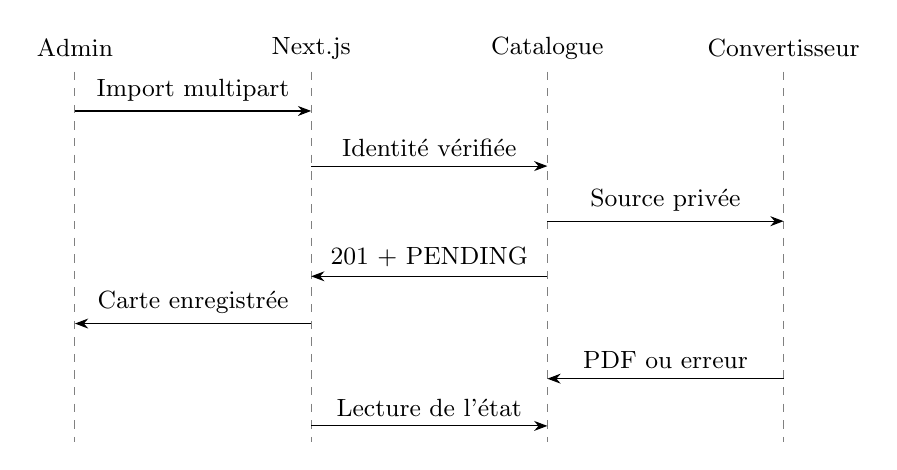
\begin{tikzpicture}[>=Stealth,font=\small]
\foreach \x/\name in {0/Admin,3/Next.js,6/Catalogue,9/Convertisseur}{\node at (\x,0){\name};\draw[dashed,gray](\x,-0.3)--(\x,-5);}
\draw[->](0,-0.8)--node[above]{Import multipart}(3,-0.8);\draw[->](3,-1.5)--node[above]{Identité vérifiée}(6,-1.5);\draw[->](6,-2.2)--node[above]{Source privée}(9,-2.2);\draw[->](6,-2.9)--node[above]{201 + PENDING}(3,-2.9);\draw[->](3,-3.5)--node[above]{Carte enregistrée}(0,-3.5);\draw[->](9,-4.2)--node[above]{PDF ou erreur}(6,-4.2);\draw[->](3,-4.8)--node[above]{Lecture de l’état}(6,-4.8);\end{tikzpicture}\caption{Séquence d’un import avec conversion différée}\end{figure}

\chapter{Modélisation et gestion des données}
\section{Relations}
User est la racine de l’identité ; Student et Administrator portent les profils et RefreshToken les sessions. Subject possède Chapter, puis Lesson et Exercise. ExerciseAttempt relie tentative, exercice et userId. Les identifiants interservices sont des références logiques : supprimer un compte demande une propagation explicite.

\begin{figure}[ht]\centering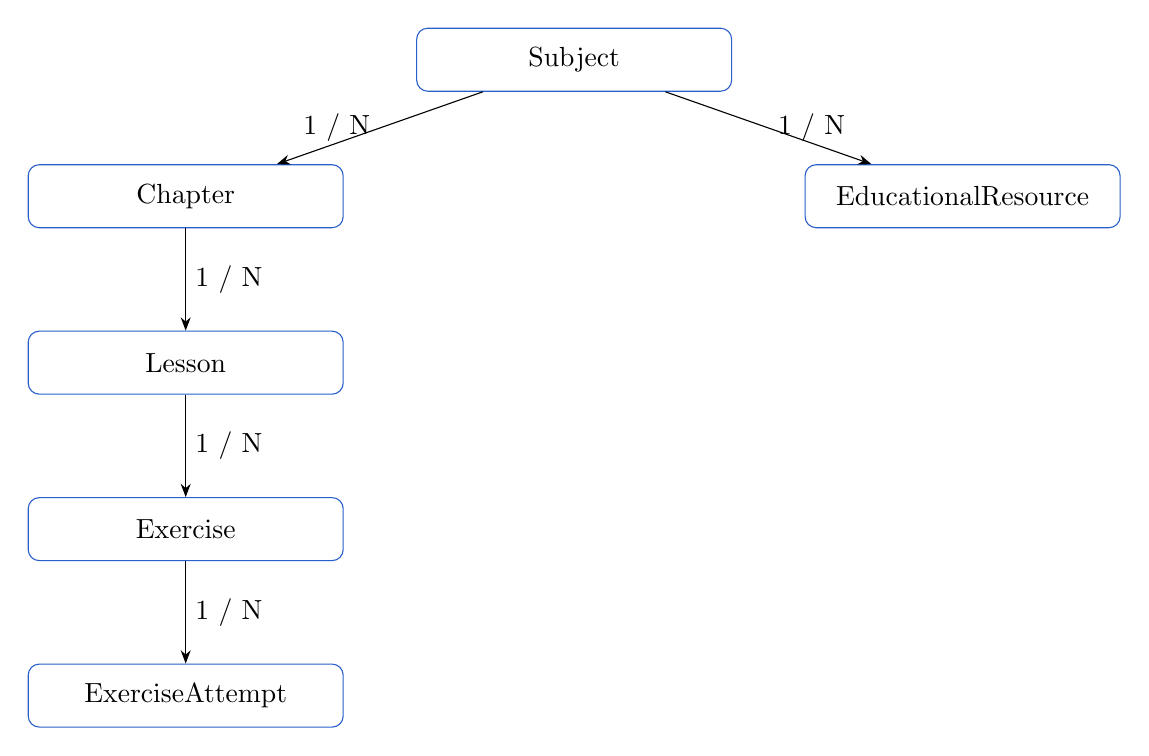
\begin{tikzpicture}[node distance=13mm,box/.style={draw=nexora,rounded corners,minimum width=4cm,minimum height=8mm},>=Stealth]
\node[box](s){Subject};\node[box,below left=of s](c){Chapter};\node[box,below right=of s](r){EducationalResource};\node[box,below=of c](l){Lesson};\node[box,below=of l](e){Exercise};\node[box,below=of e](a){ExerciseAttempt};\draw[->](s)--node[left]{1 / N}(c);\draw[->](s)--node[right]{1 / N}(r);\draw[->](c)--node[right]{1 / N}(l);\draw[->](l)--node[right]{1 / N}(e);\draw[->](e)--node[right]{1 / N}(a);\end{tikzpicture}\caption{Relations du domaine catalogue}\end{figure}
\section{Métadonnées et fichiers}
PostgreSQL conserve la description pédagogique et des clés opaques. SHA-256 identifie les sources ; ce n’est pas un hash de mot de passe. Le serveur peut contrôler un droit puis fournir un flux sans enregistrer les binaires en table. Publication et conversion sont indépendantes : un document publié peut être en préparation.

\section{Transactions et cohérence}
Inscription et rotation des jetons sont transactionnelles. Le disque ne participe pas à une transaction PostgreSQL : une panne entre écriture et insertion peut laisser un fichier orphelin. Réconciliation et purge sont donc nécessaires. revision protège la finalisation obsolète, sans constituer un verrou distribué complet.

\section{adaptive-qcm-service}
Modèles présents : QcmQuestion, QcmChoice, QcmMastery, QcmSession, QcmAnswer, QcmSpacedRepetition. Un schéma ne prouve pas l’achèvement des routes métier.

\lstinputlisting[language={}]{extraits/schema-adaptive-qcm-service.txt}
\section{admin-contact-service}
Modèles présents : ContactMessage, Notification. Un schéma ne prouve pas l’achèvement des routes métier.

\lstinputlisting[language={}]{extraits/schema-admin-contact-service.txt}
\section{analytics-streak-service}
Modèles présents : UserStreak, DailyActivityLog. Un schéma ne prouve pas l’achèvement des routes métier.

\lstinputlisting[language={}]{extraits/schema-analytics-streak-service.txt}
\section{auth-user-service}
Modèles présents : User, Student, Administrator, RefreshToken. Un schéma ne prouve pas l’achèvement des routes métier.

\lstinputlisting[language={}]{extraits/schema-auth-user-service.txt}
\section{catalog-course-service}
Modèles présents : ExternalResource, Subject, EducationalResource, Chapter, Lesson, Exercise, ExerciseAttempt, ReferenceBook. Un schéma ne prouve pas l’achèvement des routes métier.

\lstinputlisting[language={}]{extraits/schema-catalog-course-service.txt}
\section{exam-submission-service}
Modèles présents : CncExam, ExamSession, WrittenSubmission. Un schéma ne prouve pas l’achèvement des routes métier.

\lstinputlisting[language={}]{extraits/schema-exam-submission-service.txt}

\chapter{Analyse technique et compromis}
\section{Décisions observables}
L’organisation par domaines, les rôles, les clients Prisma distincts et le lecteur partagé sont observables. Aucune intention historique non enregistrée n’est attribuée à un auteur. La séparation des services favorise l’étude des domaines mais multiplie processus, ports et modes de panne.

\section{Maintenabilité}
Le tableau de bord conserve sa structure tout en recevant des propriétés serveur. Les anciens modules restent volumineux et mêlent données locales et UI. Les extraire progressivement doit conserver les comportements ; un redesign global pendant un branchement backend crée des régressions.

\section{Sécurité de conversion}
Le contenu importé reste hostile même transmis par un administrateur. Réseau, mémoire, processus et durée sont limités au niveau du moteur. Les sources sont montées en lecture seule ; le résultat transite par une sortie plafonnée. Les images et parsers doivent être actualisés.

\section{Stockage et travaux}
Le disque privé est utilisable sans bucket public mais exige sauvegardes et volume persistant. Le drapeau busy en mémoire et la reprise des travaux conviennent à une instance locale. Plusieurs réplicas nécessitent worker dédié, baux et tentatives bornées.

\section{Dette technique}
Examens, tickets et orchestration QCM restent incomplets ; certains réglages et pochettes sont locaux. Le résumé ne transforme pas toute interaction en événement. Un message de succès local ne doit jamais être présenté comme preuve d’écriture PostgreSQL.

\section{Évolutions}
Prioriser pagination, migrations versionnées, purge des orphelins, adaptateur MinIO privé et file robuste. Relier ensuite événements, sessions QCM, soumissions et tickets. Chaque évolution doit ajouter des tests de refus et de reprise, pas seulement un scénario heureux.

\chapter{Guide de développement et exploitation}
\section{Démarrage}
Configurer backend/.env depuis .env.example avec URL PostgreSQL et secrets aléatoires. Démarrer la base, générer Prisma, appliquer les schémas puis resource-constraints.sql. Construire nexora-converter:local depuis backend/converter. Lancer npm run dev dans backend et frontend. Ports : 3000, 4000 et 4001 à 4006 ; ne pas exposer les services internes publiquement.

\section{Ajouter une fonctionnalité}
Décrire entrée, sortie, rôle et invariants. Ajouter modèle et validation Zod, route dans le service propriétaire, relais Next puis composant. Pour un document privé, contrôler aussi son URL de fichier. Réutiliser cartes, boutons et lecteur au lieu de remplacer la page entière.

\section{Modifier une entité}
Définir nullabilité, valeurs par défaut et index selon les requêtes. Préciser si une suppression cascade ou est refusée. Générer le client et appliquer une migration contrôlée. Rendre un champ obligatoire exige une reprise des anciennes données.

\section{Exemple CRUD}
Publier envoie PATCH avec les métadonnées complètes. La route exige ADMIN, valide filière/année, retrouve la matière et met à jour la ligne. Le test publie, vérifie la visibilité comme étudiant, dépublie puis exige 404 par identifiant : ce dernier contrôle protège les liens conservés.

\section{Déboguer}
Une page vide demande le journal frontend. 401 concerne la session ; 403 le rôle ou l’origine ; 503 un service absent. Pour convertir, vérifier Docker, image, packages et limites sans exécuter le document sur l’hôte. Une DLL Prisma verrouillée sous Windows demande l’arrêt du service avant génération.

\section{Tester}
npm test vérifie les moteurs et fichiers ; npm run typecheck valide les workspaces. frontend utilise npx tsc --noEmit. scripts/check-resources.mjs traverse HTTP et --conversions ajoute Office/TEX. create-resource-fixtures.py produit les documents jetables. Les contrôles locaux ont vérifié les six extensions, les brouillons, rôles, filtres, téléchargements et CSRF.

\section{Sauvegarder et déployer}
Sauvegarder base et dossier privé ensemble. Garder les secrets hors de Git ; réserver les comptes publics à la démo. Configurer HTTPS et APP\_ORIGIN. Avant diffusion, préparer supervision, rotation de logs et restauration testée. Ne pas déployer plusieurs convertisseurs avec la reprise actuelle.

\begin{concept}{Erreur fréquente}TypeScript ne vérifie ni la disponibilité PostgreSQL ni la présence d’un binaire natif Tailwind. Une conversion réussie ne prouve pas les permissions : ces propriétés exigent des tests différents.\end{concept}

\chapter{Glossaire et révision}
\section*{API}
Contrat d’échange. Utilité et exemple : /api/resources relie interface et catalogue.

\section*{Middleware}
Étape de traitement HTTP. Utilité et exemple : requireUser refuse un rôle insuffisant.

\section*{DTO}
Représentation de données pour un échange. Utilité et exemple : serialize omet les clés privées.

\section*{ORM}
Correspondance objets/tables. Utilité et exemple : Prisma fournit findMany.

\section*{Transaction}
Modifications atomiques. Utilité et exemple : Compte et jetons sont créés ensemble.

\section*{Index}
Structure accélérant une recherche. Utilité et exemple : Le catalogue indexe ses critères.

\section*{Clé étrangère}
Référence garantie par la base. Utilité et exemple : subjectId référence Subject.

\section*{JWT}
Assertions signées. Utilité et exemple : La gateway vérifie rôle et signature.

\section*{Hash}
Empreinte irréversible. Utilité et exemple : SHA-256 protège le refresh token stocké.

\section*{Sel}
Aléa du hachage de mot de passe. Utilité et exemple : Bcrypt produit des hashes distincts pour un même secret.

\section*{CSRF}
Requête indésirable utilisant la session. Utilité et exemple : Origin est vérifié sur les mutations.

\section*{XSS}
Exécution de contenu injecté. Utilité et exemple : MathFormula garde un fallback texte.

\section*{CORS}
Règles navigateur interorigines. Utilité et exemple : La gateway déclare les origines.

\section*{Sandbox}
Environnement à capacités limitées. Utilité et exemple : Le convertisseur n’a pas de réseau.

\section*{Tmpfs}
Espace temporaire en mémoire. Utilité et exemple : La conversion dispose de 256 Mo.

\section*{Cache}
Réutilisation d’un résultat. Utilité et exemple : outputKey désigne le PDF conservé.

\section*{Idempotence}
Même effet après répétition. Utilité et exemple : Les seeds utilisent des upserts.

\section*{Révision}
Version d’un état métier. Utilité et exemple : revision refuse un résultat obsolète.

\section*{Hydratation}
Activation client du rendu serveur. Utilité et exemple : React connecte les boutons du dashboard.

\section*{État vide}
Vue d’absence de résultat. Utilité et exemple : Le catalogue invite à changer les filtres.

\section*{Streak}
Série de jours actifs. Utilité et exemple : Le résumé compare le dernier jour au jour courant.

\section*{Polling}
Interrogation périodique. Utilité et exemple : ResourceReader attend READY.

\section{Questions à résoudre dans le code}
Pourquoi vérifier les droits sur le fichier si sa carte était protégée ? Pourquoi le temps de travail ne mesure-t-il pas la maîtrise ? Pourquoi un document publié peut-il être en préparation ? Pourquoi une transaction SQL ne supprime-t-elle pas un fichier orphelin ? Retrouver la fonction puis proposer un test de refus ou de reprise pour chaque cas.

\bibliographystyle{plain}\nocite{*}\bibliography{references}\end{document}
